\ifdefined\CUMULATIVEPRACTICE
\else
\documentclass[11pt]{article}

\usepackage[utf8]{inputenc}
\usepackage[T1]{fontenc}
\usepackage{lmodern}
\usepackage[margin=1in]{geometry}
\usepackage[dvipsnames]{xcolor}
\usepackage{graphicx, booktabs, enumitem, float, framed, caption, multirow}
\usepackage{fancyhdr}
\usepackage{tcolorbox}
\usepackage{listings}
\usepackage{tikz}
\usepackage{setspace}
\usepackage{needspace}
\IfFileExists{algorithm.sty}{%
  \usepackage{algorithm}
  \usepackage[noend]{algpseudocode}
  \newcommand{\hasalgorithms}{}%
}{}
\usepackage{amsmath,amssymb,bm,xcolor}



\newcommand{\act}{a}                    %
\newcommand{\actspace}{\mathcal{A}}     %
\newcommand{\Sset}{\mathcal{S}}         %


\newcommand{\bel}{\mathrm{bel}}         %
\newcommand{\cellbelief}{B}            %

\newcommand{\rot}{\mathbf{R}}           %
\newcommand{\tra}{\mathbf{t}}           %
\newcommand{\Tf}[2]{{}^{#1}\mathbf{T}_{#2}}  %
\usepackage{hyperref}

\definecolor{DartmouthGreen}{HTML}{00693E}
\newcommand{\dgreen}[1]{\textcolor{DartmouthGreen}{#1}}
\newcommand{\dgbf}[1]{\textbf{\dgreen{#1}}}      %
\urlstyle{same}
\hypersetup{
    colorlinks=true,
    linkcolor=DartmouthGreen,
    filecolor=DartmouthGreen,
    citecolor=DartmouthGreen,
    urlcolor=DartmouthGreen,
    breaklinks=true
}

\newcommand{\coursenumber}{COSC 81/281}
\newcommand{\gradescopelink}{\textbf{Gradescope} (\url{https://www.gradescope.com/courses/1372528})}


\setlength{\parindent}{0pt}
\setlength{\parskip}{6pt plus 2pt minus 1pt}
\setlength{\headheight}{13.6pt}
\setlength{\emergencystretch}{3em}
\setcounter{secnumdepth}{0}

\DeclareRobustCommand{\callout}[2][gray!10]{%
  \begin{tcolorbox}[left=8pt, arc=0pt, outer arc=0pt,
                    colframe=#1, colback=#1, coltext=black]#2\end{tcolorbox}}




\newcommand{\gradstar}{$\bigstar$~\textsf{\small (required for 281; optional for 81)}~}
\newcommand{\bonusq}{\textsf{\small\textbf{[Bonus]}}~}
\newcommand{\bonus}{\bonusq}

\newcommand{\setupheader}[1]{%
  \fancypagestyle{default}{%
      \lhead{#1}
      \chead{}
      \rhead{\textbf{\coursenumber}}
      \lfoot{}
      \cfoot{}
      \rfoot{\thepage}
      \renewcommand{\headrulewidth}{0.4pt}
      \renewcommand{\footrulewidth}{0.4pt}
  }
  \pagestyle{default}
  \fancypagestyle{plain}{\pagestyle{default}}
}
\newcommand{\setupexamheader}[1]{%
  \fancypagestyle{default}{%
      \lhead{#1}
      \chead{Name:}
      \rhead{}
      \lfoot{}
      \cfoot{}
      \rfoot{\thepage}
      \renewcommand{\headrulewidth}{0.4pt}
      \renewcommand{\footrulewidth}{0.4pt}
  }
  \pagestyle{default}
  \fancypagestyle{plain}{\pagestyle{default}}
}
\newcommand{\pstitle}[2]{%
  \title{\textbf{\coursenumber:} #1}
  \author{\textbf{Due} #2\\
  }
  \date{}
}

\newcommand{\coursenotice}{%
  \callout{Problem sets are graded \textbf{pass/fail on completion}, and
  there are no late days. The problem sets are where the learning happens,
  and they are the best available practice for the midterm and final exam.
  Submit to \gradescopelink\ and assign each question to a page in your
  submission. Questions are welcome on \dgbf{Slack}. Starred ($\bigstar$)
  questions are required for COSC 281 students and optional (ungraded) for
  COSC 81 students.}}

\lstset{
  language=python,
  basicstyle=\ttfamily,
  commentstyle=\color{BrickRed},
  stringstyle=\color{ForestGreen},
  showstringspaces=false,
  breaklines=true,
  breakatwhitespace=true,
  keywordstyle=\color{Purple},
  emph={def},
  emphstyle=\color{RoyalBlue}
}
\lstnewenvironment{itemlisting}[1][]
 {\mbox{}\vspace*{-\baselineskip}%
  \lstset{xleftmargin=\leftmargin, linewidth=\linewidth, #1}}
 {}

\makeatletter
\def\fps@figure{htbp}
\makeatother
\ifdefined\hasalgorithms
\fi


\newenvironment{studentanswer}[1]
  {\par\medskip\noindent
   \begin{tcolorbox}[height from=#1 to 100cm, colback=white, colframe=gray!60,
     boxrule=0.6pt, arc=0pt, outer arc=0pt, left=7pt, right=7pt,
     top=7pt, bottom=7pt, title={Answer / work}, fonttitle=\small,
     coltitle=black, colbacktitle=gray!8, titlerule=0pt]
   \ignorespaces}
  {\end{tcolorbox}\par}


\setupexamheader{\coursenumber\ -- Final Practice}
\graphicspath{{final-practice/}}
\begin{document}
\begin{framed}
This is an untimed collection of practice problems for the cumulative
final. It is not intended to match the exam's length, point distribution,
or order of questions. Work through the problems before consulting the
solutions. Show calculations and explain the reasoning behind conceptual
answers. More than one approach may be valid when its assumptions are
clearly stated and justified.
\end{framed}
\clearpage
\section*{Formulas}
\begingroup
\small
\setlength{\abovedisplayskip}{4pt}
\setlength{\belowdisplayskip}{4pt}
\textbf{Search and planning}
\[
 f(n)=g(n)+h(n),\quad h(n)\le h^*(n),\quad
 h(n)\le c(n,n')+h(n'),\quad h(G)=0
\]

\textbf{MDPs and RL}
\[
 (\Sset,\actspace,T,R,\gamma),\quad T(s'\mid s,a)=P(s'\mid s,a),\quad
 \sum_{s'}T(s'\mid s,a)=1,\quad 0\le\gamma<1
\]
\[
 \begin{gathered}
 Q^*(s,a)=\sum_{s'}T(s'\mid s,a)
 [R(s,a,s')+\gamma\max_{a'}Q^*(s',a')]\\[4pt]
 V^*(s)=\max_a Q^*(s,a),\qquad
 \pi^*(s)\in\arg\max_a Q^*(s,a)
 \end{gathered}
\]
\[
 V_{k+1}(s)=\max_a\sum_{s'}T(s'\mid s,a)[R(s,a,s')+\gamma V_k(s')]
\]
\[
 V^{\pi_k}(s)=\sum_{s'}T(s'\mid s,\pi_k(s))
 [R(s,\pi_k(s),s')+\gamma V^{\pi_k}(s')]
\]
\[
 \pi_{k+1}(s)\in\arg\max_a\sum_{s'}T(s'\mid s,a)[R(s,a,s')+\gamma V^{\pi_k}(s')]
\]
\[
 V(s)\leftarrow V(s)+\alpha[r+\gamma V(s')-V(s)]
\]
\[
 Q(s,a)\leftarrow Q(s,a)+\alpha[r+\gamma\max_{a'}Q(s',a')-Q(s,a)]
\]
\textbf{Optimization}
\[
 x_{k+1}=x_k-\alpha f'(x_k),\qquad
 f(x)\approx f(x_0)+f'(x_0)(x-x_0)+\tfrac12 f''(x_0)(x-x_0)^2
\]
\[
 F(x)=\frac1N\sum_{i=1}^N f_i(x),\quad
 F'(x)=\frac1N\sum_{i=1}^N f_i'(x),\quad
 \widehat g(x)=\frac1m\sum_{j=1}^m f_{i_j}'(x)\approx F'(x)
\]
\textbf{Transforms}
\[
 \Tf{a}{b}=\begin{bmatrix}\rot&\tra\\0&1\end{bmatrix},\quad
 \begin{bmatrix}p_a\\1\end{bmatrix}=\Tf{a}{b}\begin{bmatrix}p_b\\1\end{bmatrix},\quad
 \Tf{a}{c}=\Tf{a}{b}\Tf{b}{c},\quad
 R_z(\theta)=\begin{bmatrix}\cos\theta&-\sin\theta&0\\\sin\theta&\cos\theta&0\\0&0&1\end{bmatrix}
\]
\textbf{Calculus}
\[
 (x^n)'=nx^{n-1},\quad(\sin x)'=\cos x,\quad(\cos x)'=-\sin x
\]
\[
 \sin0=0,\quad\cos0=1,\quad\sin(\pi/2)=1,\quad\cos(\pi/2)=0
\]
\textbf{Beliefs and filtering}
\[
 B_t(x_i)=P(X_t=x_i\mid z_{0:t},u_{1:t}),\qquad
 P(x_i\mid z)=\frac{P(z\mid x_i)P(x_i)}
 {\sum_jP(z\mid x_j)P(x_j)}
\]
\[
 \overline B_t(x_i)=\sum_j T(x_i\mid x_j,u_t)B_{t-1}(x_j)
\]
\[
 \widetilde B_t(x_i)=P(z_t\mid x_i)\overline B_t(x_i),\qquad
 B_t(x_i)=\frac{\widetilde B_t(x_i)}{\sum_j\widetilde B_t(x_j)}
\]
\endgroup

\clearpage
\fi

\section*{Question 1: Following and modifying a heuristic}
The directed graph has edges $S\to U$ of cost 4, $S\to V$ of cost 1,
$V\to U$ of cost 1, $U\to G$ of cost 2, and $V\to G$ of cost 6.
There are no other edges. The heuristic at $(S,U,V,G)$ is $(4,2,3,0)$.
A* selects the smallest $g+h$, breaking ties by smaller $h$, then
alphabetical label. Reopen a node when its path cost improves, and stop
when the goal is selected.
\begin{center}
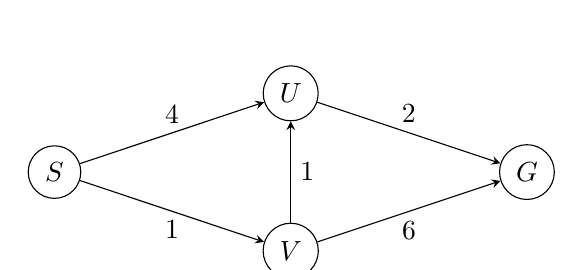
\begin{tikzpicture}[>=stealth]
\node[circle,draw] (S) at (0,0){$S$};
\node[circle,draw] (U) at (3,1){$U$};
\node[circle,draw] (V) at (3,-1){$V$};
\node[circle,draw] (G) at (6,0){$G$};
\draw[->] (S)--node[above]{4}(U);
\draw[->] (S)--node[below]{1}(V);
\draw[->] (V)--node[right]{1}(U);
\draw[->] (U)--node[above]{2}(G);
\draw[->] (V)--node[below]{6}(G);
\end{tikzpicture}
\end{center}
\begin{enumerate}[label=(\alph*)]
\item \begin{minipage}[t]{\linewidth} Trace A* through goal selection. Give the frontier priorities after
each nonterminal expansion and the returned path.

\begin{studentanswer}{5cm}
%%%%% SOLUTION HERE %%%%%
\end{studentanswer}

\end{minipage}
\item \begin{minipage}[t]{\linewidth} Change only $h(V)$ to 2. Determine admissibility and consistency.
If they differ, explain how that is possible.

\begin{studentanswer}{4cm}
%%%%% SOLUTION HERE %%%%%
\end{studentanswer}

\end{minipage}
\end{enumerate}

\clearpage
\section*{Question 2: Steering a robot with a footprint}
A rectangular robot translates without rotating. Its width is 1 along
$x$ and its height is 2 along $y$. Its configuration is its center.
An obstacle occupies $[2,3]\times[2,3]$. Contact counts as collision.
An RRT has nodes $q_0=(0,0)$ and $q_1=(0,2)$ and samples $q_s=(4,2)$.
Use Euclidean nearest-node selection and straight-line steering.
\begin{center}
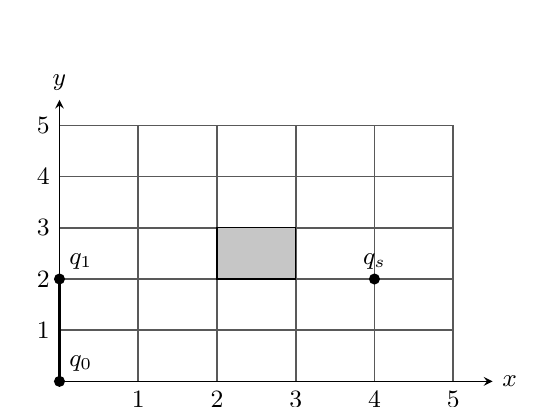
\begin{tikzpicture}[x=1cm,y=.65cm,>=stealth,font=\small]
\draw[step=1,black!65,line width=.6pt] (0,0) grid (5,5);
\draw[->] (0,0)--(5.5,0) node[right]{$x$};
\draw[->] (0,0)--(0,5.5) node[above]{$y$};
\foreach \x in {1,2,3,4,5}\node[below] at (\x,0){\x};
\foreach \y in {1,2,3,4,5}\node[left] at (0,\y){\y};
\filldraw[fill=gray!45] (2,2) rectangle (3,3);
\draw[thick] (0,0)--(0,2);
\fill (0,0) circle(2pt) node[above right]{$q_0$};
\fill (0,2) circle(2pt) node[above right]{$q_1$};
\fill (4,2) circle(2pt) node[above]{$q_s$};

\end{tikzpicture}
\end{center}
\begin{enumerate}[label=(\alph*)]
\item \begin{minipage}[t]{\linewidth} Draw and state the set of center positions in collision.
Which node is nearest to the sample?

\begin{studentanswer}{3.5cm}
%%%%% SOLUTION HERE %%%%%
\end{studentanswer}

\end{minipage}
\item \begin{minipage}[t]{\linewidth} Starting independently from the original tree, test maximum
extension lengths 1 and 4. Give each endpoint and whether the extension
is accepted. Explain why endpoint testing is insufficient.

\begin{studentanswer}{4cm}
%%%%% SOLUTION HERE %%%%%
\end{studentanswer}

\end{minipage}
\end{enumerate}

\clearpage
\section*{Question 3: Two ways to improve a policy}
An MDP has nonterminal states $A,B$ and terminal state $Z$.
At $A$, stop gives reward 2 and terminates; continue gives reward 0
and enters $B$. At $B$, finish gives reward 6 and terminates.
Use $\gamma=1/2$ and terminal value zero.
\begin{enumerate}[label=(\alph*)]
\item \begin{minipage}[t]{\linewidth} Starting with $V_0=0$, perform two synchronous VI sweeps.
Show the candidate action values at $A$ in each sweep.

\begin{studentanswer}{4cm}
%%%%% SOLUTION HERE %%%%%
\end{studentanswer}

\end{minipage}
\item \begin{minipage}[t]{\linewidth} Start PI from the policy that stops at $A$. Evaluate it exactly,
then improve it. Is the improved policy already optimal here? Explain.

\begin{studentanswer}{4cm}
%%%%% SOLUTION HERE %%%%%
\end{studentanswer}

\end{minipage}
\end{enumerate}

\clearpage
\section*{Question 4: A model and two estimates from the same episodes}
A fixed policy produced two complete episodes,
\[
 A\xrightarrow{1}B\xrightarrow{2}Z,\qquad A\xrightarrow{3}Z.
\]
State $Z$ is terminal. Use $\gamma=1/2$.
\begin{enumerate}[label=(\alph*)]
\item \begin{minipage}[t]{\linewidth} Estimate transition probabilities for this policy by counting
observed transitions. Give the reward for each observed transition type,
then solve for the values in this empirical model.

\begin{studentanswer}{4cm}
%%%%% SOLUTION HERE %%%%%
\end{studentanswer}

\end{minipage}
\item \begin{minipage}[t]{\linewidth} Compute direct-evaluation estimates by averaging observed returns.
Then process the episodes in their given order with TD, starting at zero
and using learning rate $1/2$. Show each update.

\begin{studentanswer}{5cm}
%%%%% SOLUTION HERE %%%%%
\end{studentanswer}

\end{minipage}
\item \begin{minipage}[t]{\linewidth} Explain why the results do not establish that the policy is optimal.

\begin{studentanswer}{3cm}
%%%%% SOLUTION HERE %%%%%
\end{studentanswer}

\end{minipage}
\end{enumerate}

\clearpage
\section*{Question 5: Learning action values from a short log}
Initialize every Q-entry to zero. Use $\alpha=\gamma=1/2$ and process
these records in order. $Z$ is terminal.
\begin{center}
\begin{tabular}{cccc}
\toprule State & Action & Reward & Next state\\\midrule
$S$ & left & 2 & $A$\\
$A$ & finish & 4 & $Z$\\
$S$ & left & 0 & $A$\\\bottomrule
\end{tabular}
\end{center}
\begin{enumerate}[label=(\alph*)]
\item \begin{minipage}[t]{\linewidth} Compute the Q-learning sample and new table entry for each record.
All unlisted entries remain zero.

\begin{studentanswer}{5cm}
%%%%% SOLUTION HERE %%%%%
\end{studentanswer}

\end{minipage}
\item \begin{minipage}[t]{\linewidth} An untried action right at $S$ still has value zero. Does the
greedy choice prove left is better? Would a larger learning rate supply
the missing evidence?

\begin{studentanswer}{4cm}
%%%%% SOLUTION HERE %%%%%
\end{studentanswer}

\end{minipage}
\end{enumerate}

\clearpage
\section*{Question 6: A local model and sampled gradient steps}
Let $f(x)=e^x+x^2-3x$. Construct its quadratic Taylor model $m(x)$
about $x_0=0$. Use this same model for all updates below.
\begin{enumerate}[label=(\alph*)]
\item \begin{minipage}[t]{\linewidth} Compute $f(0)$, $f'(0)$, and $f''(0)$, then write $m(x)$.

\begin{studentanswer}{4cm}
%%%%% SOLUTION HERE %%%%%
\end{studentanswer}

\end{minipage}
\item \begin{minipage}[t]{\linewidth} Starting at $x=1$, take one gradient-descent step on $m$
with learning rate $\alpha=1/2$. Compute the model's value before and
after the step. Use $m'$, not $f'$, for this update.

\begin{studentanswer}{4cm}
%%%%% SOLUTION HERE %%%%%
\end{studentanswer}

\end{minipage}
\item \begin{minipage}[t]{\linewidth} Instead of using $m'(1)$, suppose a sampled update uses
one of the supplied gradient estimates $g_1=-1$ and $g_2=3$, each with
probability $1/2$. Starting separately from $x=1$ in each case,
compute the two updates $x_{\mathrm{sample}}=1-\alpha g_i$ using
the same $\alpha=1/2$. Compare their average with part (b).
Does either individual update have to equal the full-gradient update?

\begin{studentanswer}{5cm}
%%%%% SOLUTION HERE %%%%%
\end{studentanswer}

\end{minipage}
\end{enumerate}

\clearpage
\section*{Question 7: Composing frames along an arm}
A base frame $b$ is rotated $90^\circ$ about world $z$ and translated
by $(1,2,0)$ in the world. A link frame $\ell$ has the same orientation
as the base and origin $(2,0,0)$ in the base frame. Its tip has link-frame
coordinates $(1,0,0)$.
\begin{enumerate}[label=(\alph*)]
\item \begin{minipage}[t]{\linewidth} Write both $4\times4$ transforms, compose them, and compute the
tip's world coordinates. Label the source and destination frames.

\begin{studentanswer}{6cm}
%%%%% SOLUTION HERE %%%%%
\end{studentanswer}

\end{minipage}
\item \begin{minipage}[t]{\linewidth} Why is adding $(1,2,0)+(2,0,0)+(1,0,0)$ incorrect?

\begin{studentanswer}{3.5cm}
%%%%% SOLUTION HERE %%%%%
\end{studentanswer}

\end{minipage}
\end{enumerate}

\clearpage
\section*{Question 8: Choosing methods from available information}
Consider A*, PRM, RRT, VI, PI, fixed-policy V-learning, Q-learning,
and trajectory optimization. Several proposals may be defensible.
For each setting, recommend an approach, explain why the available
information supports it, and identify one limitation. Two or three
sentences per setting are sufficient. You may combine methods.
\begin{enumerate}[label=(\alph*)]
\item \begin{minipage}[t]{\linewidth} A robot receives many start-goal requests in a known static
building. Collision checking is available and preprocessing is allowed.
\emph{Hint: Consider what could be built once and reused, and how a route
would be found within that representation.}

\begin{studentanswer}{4cm}
%%%%% SOLUTION HERE %%%%%
\end{studentanswer}

\end{minipage}
\item \begin{minipage}[t]{\linewidth} Actions have uncertain outcomes. A small finite transition and
reward model is known, and a policy is needed for every state. Later,
only recorded episodes under one fixed policy are available.
Recommend a method for the known-model setting and a method for estimating
the recorded policy's value.
\emph{Hint: Distinguish improving a policy from evaluating one. Which
methods need a transition model, and which can use observed experience?}

\begin{studentanswer}{4cm}
%%%%% SOLUTION HERE %%%%%
\end{studentanswer}

\end{minipage}
\item \begin{minipage}[t]{\linewidth} A geometric route is known, but executing it produces abrupt
motions and violates acceleration limits. A dynamics model is available.
\emph{Hint: The route is already known. Consider a method that can adjust
its timing and motion while accounting for actuator constraints.}

\begin{studentanswer}{4cm}
%%%%% SOLUTION HERE %%%%%
\end{studentanswer}

\end{minipage}
\end{enumerate}

\clearpage
\section*{Question 9: Filtering in a long aisle}
A robot drives through a long straight aisle with identical parallel
walls. Its lidar sees the side walls but neither end of the aisle and
no distinctive features along its length. The robot uses wheel odometry
and lidar in an EKF with nonlinear motion and measurement models.
Its lateral position is well localized, but uncertainty about its progress
along the aisle grows.
\begin{enumerate}[label=(\alph*)]
\item \begin{minipage}[t]{\linewidth} Explain how the filter uses a motion command to predict the
pose belief, then uses a lidar reading to correct it. Why should a
difference between predicted and measured range not be treated entirely
as pose error?

\begin{studentanswer}{4cm}
%%%%% SOLUTION HERE %%%%%
\end{studentanswer}

\end{minipage}
\item \begin{minipage}[t]{\linewidth} Explain why the scan can constrain the lateral position but
not progress along the aisle. Would replacing the EKF with a UKF, or
adding more particles to a particle filter, necessarily resolve this
uncertainty? Give one measurement that would provide the missing information.

\begin{studentanswer}{5cm}
%%%%% SOLUTION HERE %%%%%
\end{studentanswer}

\end{minipage}
\end{enumerate}
\clearpage
\noindent\textbf{Question 9 (continued)}
\begin{enumerate}[label=(\alph*),start=3]
\item \begin{minipage}[t]{\linewidth} \gradstar Suppose the pose belief is concentrated near a good
estimate. Compare how an EKF and a UKF propagate it through a nonlinear
model, giving one benefit and one limitation of each. Does Gaussian
noise make either method exact for every nonlinear model?
No equations or derivations are required.

\begin{studentanswer}{5cm}
%%%%% SOLUTION HERE %%%%%
\end{studentanswer}

\end{minipage}
\end{enumerate}

\clearpage
\section*{Question 10: Planning Scenarios}
Sketch a two-dimensional environment in which A* on a sufficiently fine
grid could find a route more reliably within a fixed computation budget
than a basic RRT with uniform sampling and 5\% goal bias. Identify the
start, goal, and obstacles. Explain what makes the environment difficult
for RRT, then describe a change that could reduce that difficulty.
State any assumptions needed for the grid comparison.

\begin{studentanswer}{9cm}
%%%%% SOLUTION HERE %%%%%
\end{studentanswer}

\clearpage
\section*{Question 11: Two modes and their average}
A robot is equally likely to be near position $x=-3$ or $x=3$ along
a corridor. Each cluster is narrow, and the region near $x=0$ is a wall.
The sketch shows the qualitative posterior density.
\begin{center}
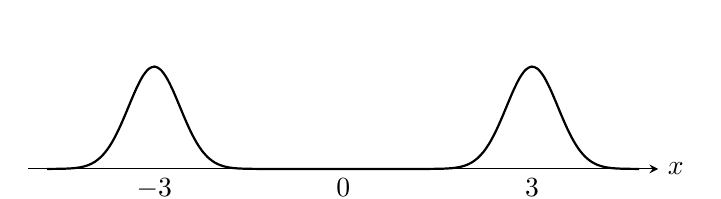
\begin{tikzpicture}[x=.8cm,y=1cm,>=stealth]
\draw[->] (-5,0)--(5,0) node[right]{$x$};
\draw[thick,domain=-4.7:4.7,samples=100,smooth]
 plot (\x,{1.3*exp(-3*(\x+3)^2)+1.3*exp(-3*(\x-3)^2)});
\foreach \x in {-3,0,3}\node[below] at (\x,0){$\x$};
\end{tikzpicture}
\end{center}
\begin{enumerate}[label=(\alph*)]
\item \begin{minipage}[t]{\linewidth} What does the posterior mean report? Explain why reporting only
that point can be misleading. Can a single Gaussian faithfully represent
the two narrow peaks?

\begin{studentanswer}{4cm}
%%%%% SOLUTION HERE %%%%%
\end{studentanswer}

\end{minipage}

\item \begin{minipage}[t]{\linewidth} Compare a standard single-Gaussian UKF with a particle filter
for this belief. What can cause a particle filter to lose an important
hypothesis, and what does the UKF's use of sigma points not imply?

\begin{studentanswer}{4cm}
%%%%% SOLUTION HERE %%%%%
\end{studentanswer}

\end{minipage}

\end{enumerate}

\clearpage
\section*{Question 12: Motion, evidence, and a normalized belief}
A robot occupies one of three cells. A door is present only in cell 3.
Model its hidden cell as an HMM. The next cell depends only on the
current cell and motion command, and the reading depends only on the
cell occupied when it is taken.
Its current belief is
$(\cellbelief(x_1),\cellbelief(x_2),\cellbelief(x_3))=(1/2,1/4,1/4)$,
where $x_i$ denotes occupancy of cell $i$.
\begin{center}
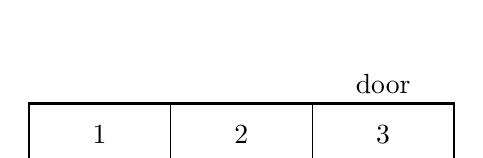
\begin{tikzpicture}[x=1.8cm,y=.8cm]
\draw[thick] (0,0) rectangle (3,1);
\draw (1,0)--(1,1) (2,0)--(2,1);
\node at (.5,.5){1}; \node at (1.5,.5){2};
\node at (2.5,.5){3};
\node[above] at (2.5,1){door};
\end{tikzpicture}
\end{center}
The robot first attempts to move right. From cells 1 and 2 it moves
one cell right with probability $1/2$ and stays with probability $1/2$.
From cell 3 it stays with probability 1. It then receives a
\texttt{door} reading, whose likelihood is $1/4$ in cells 1 and 2,
and $3/4$ in cell 3.
\begin{enumerate}[label=(\alph*)]
\item \begin{minipage}[t]{\linewidth} Apply only the motion update. Fill every cell of the first row
below with its predicted probability $\overline{\cellbelief}(x_i)$.
Do not use the \texttt{door} reading in this part. Show which previous cells
contribute to each entry.

\begin{studentanswer}{4cm}
%%%%% SOLUTION HERE %%%%%
\begin{center}\begin{tabular}{|p{2cm}|p{2cm}|p{2cm}|}\hline
Cell 1 & Cell 2 & Cell 3\\\hline
\rule{0pt}{.8cm}&&\\\hline\end{tabular}\end{center}
\end{studentanswer}

\end{minipage}
\item \begin{minipage}[t]{\linewidth} Multiply the predicted probability in each cell by that cell's
likelihood for the observed reading. Fill the row with these
unnormalized weights $\widetilde{\cellbelief}(x_i)$ and compute their sum.

\begin{studentanswer}{4cm}
%%%%% SOLUTION HERE %%%%%
\begin{center}\begin{tabular}{|p{2cm}|p{2cm}|p{2cm}|}\hline
Cell 1 & Cell 2 & Cell 3\\\hline
\rule{0pt}{.8cm}&&\\\hline\end{tabular}\end{center}
\end{studentanswer}

\end{minipage}
\end{enumerate}
\clearpage
\noindent\textbf{Question 12 (continued)}
\begin{enumerate}[label=(\alph*),start=3]
\item \begin{minipage}[t]{\linewidth} Normalize the three weights to obtain $\cellbelief_{\mathrm{new}}(x_i)$
and fill every cell below. Leave
the results as fractions. Explain why the posterior is not obtained
by normalizing the three sensor likelihoods alone.

\begin{studentanswer}{5cm}
%%%%% SOLUTION HERE %%%%%
\begin{center}\begin{tabular}{|p{2cm}|p{2cm}|p{2cm}|}\hline
Cell 1 & Cell 2 & Cell 3\\\hline
\rule{0pt}{.8cm}&&\\\hline\end{tabular}\end{center}
\end{studentanswer}

\end{minipage}
\end{enumerate}
\clearpage
\section*{Question 13: Particles and probability in each cell}
Four equally weighted particles occupy cells $(1,1,2,4)$ of a
four-cell row. A motion rule moves each particle one cell to the right,
except that a particle in cell 4 moves one cell left. For this exercise
the motion is deterministic. After the move, the likelihood of the
observed reading in cells $(1,2,3,4)$ is $(1/2,1/4,3/4,1/2)$.
\begin{center}
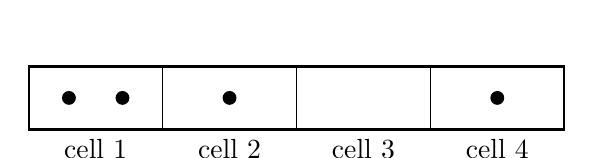
\begin{tikzpicture}[x=1.7cm,y=.8cm]
\draw[thick] (0,0) rectangle (4,1);
\foreach \x in {1,2,3}\draw (\x,0)--(\x,1);
\foreach \x/\n in {.5/1,1.5/2,2.5/3,3.5/4}\node[below] at (\x,0){cell \n};
\fill (.3,.5) circle(2.5pt); \fill (.7,.5) circle(2.5pt);
\fill (1.5,.5) circle(2.5pt); \fill (3.5,.5) circle(2.5pt);
\end{tikzpicture}
\end{center}
\begin{enumerate}[label=(\alph*)]
\item \begin{minipage}[t]{\linewidth} Draw the particles after motion in the empty row. How much
predicted probability mass is represented in each cell?

\begin{studentanswer}{3.5cm}
%%%%% SOLUTION HERE %%%%%
\begin{center}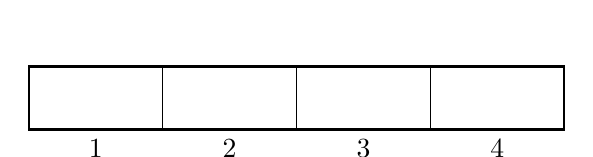
\begin{tikzpicture}[x=1.7cm,y=.8cm]
\draw[thick] (0,0) rectangle (4,1);
\foreach \x in {1,2,3}\draw (\x,0)--(\x,1);
\foreach \x/\n in {.5/1,1.5/2,2.5/3,3.5/4}\node[below] at (\x,0){\n};
\end{tikzpicture}\end{center}
\end{studentanswer}

\end{minipage}
\item \begin{minipage}[t]{\linewidth} Multiply each particle's weight by its new cell's likelihood.
Then sum the weights within each cell. Enter the unnormalized
\emph{cell masses}, not the weight of one particle, in the row below.

\begin{studentanswer}{3.5cm}
%%%%% SOLUTION HERE %%%%%
\begin{center}\begin{tabular}{|p{1.5cm}|p{1.5cm}|p{1.5cm}|p{1.5cm}|}\hline
Cell 1 & Cell 2 & Cell 3 & Cell 4\\\hline
\rule{0pt}{.8cm}&&&\\\hline\end{tabular}\end{center}
\end{studentanswer}

\end{minipage}
\end{enumerate}
\clearpage
\noindent\textbf{Question 13 (continued)}
\begin{enumerate}[label=(\alph*),start=3]
\item \begin{minipage}[t]{\linewidth} Normalize the cell masses and write them as fractions in the
row. Next, draw four particles independently with replacement from the
current particles, with selection probabilities given by their normalized
weights. Each new particle must copy an existing location. What is the
expected number in each cell? Must every set of draws produce those counts?

\begin{studentanswer}{5cm}
%%%%% SOLUTION HERE %%%%%
\begin{center}\begin{tabular}{|p{1.5cm}|p{1.5cm}|p{1.5cm}|p{1.5cm}|}\hline
Cell 1 & Cell 2 & Cell 3 & Cell 4\\\hline
\rule{0pt}{.8cm}&&&\\\hline\end{tabular}\end{center}
\end{studentanswer}

\end{minipage}
\end{enumerate}
\clearpage
\section*{Question 14: Channels, pooling, and a fully connected layer}
An RGB image has shape $6\times6\times3$. Its three channels contain
red, green, and blue values. A convolutional layer applies four learned
filters with spatial size $3\times3$, stride 1, and no padding.
Stride 1 moves each filter one pixel at a time. Count only positions
where the entire filter fits inside the image.
Each filter combines information from all three input channels and
produces one output channel. These learned channels need not represent
colors. A max-pooling layer next replaces each nonoverlapping
$2\times2$ block in each channel with its largest entry.
\begin{enumerate}[label=(\alph*)]
\item \begin{minipage}[t]{\linewidth} Determine the output dimensions after convolution and after
pooling. Explain which operation changes the number of channels and
which reduces the spatial dimensions without combining channels.

\begin{studentanswer}{4cm}
%%%%% SOLUTION HERE %%%%%
\end{studentanswer}

\end{minipage}

\item \begin{minipage}[t]{\linewidth} Pool this $4\times4$ response from one channel. Fill the
$2\times2$ output grid. Give one piece of information the output loses.
\[
\begin{bmatrix}1&3&2&0\\4&2&1&5\\0&6&3&2\\1&2&7&4\end{bmatrix}.
\]

\begin{studentanswer}{4cm}
%%%%% SOLUTION HERE %%%%%
\begin{center}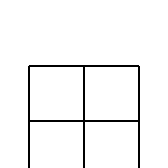
\begin{tikzpicture}
\draw[step=.7,black,line width=.7pt] (0,0) grid (1.4,1.4);
\end{tikzpicture}\end{center}
\end{studentanswer}

\end{minipage}
\end{enumerate}
\clearpage
\noindent\textbf{Question 14 (continued)}
\begin{enumerate}[label=(\alph*),start=3]
\item \begin{minipage}[t]{\linewidth} Flatten all pooled channels into a list $x_1,\ldots,x_N$.
Flattening only rearranges values. A fully connected layer has three
outputs, each computed as $y_j=\sum_{i=1}^Nw_{ji}x_i+b_j$.
Find $N$ and count the weights and biases in this layer.
Count neither convolution parameters nor arithmetic operations.

\begin{studentanswer}{5cm}
%%%%% SOLUTION HERE %%%%%
\end{studentanswer}

\end{minipage}
\end{enumerate}
\clearpage
\section*{Question 15: A supplied smoothing kernel}
Apply the following kernel to the center of the given patch:
\[
K=\frac1{16}\begin{bmatrix}1&2&1\\2&4&2\\1&2&1\end{bmatrix},
\qquad I=\begin{bmatrix}2&2&2\\2&10&2\\2&2&2\end{bmatrix}.
\]
Multiply corresponding kernel and patch entries and sum. You do not need
to recall any named kernel from memory.
\begin{enumerate}[label=(\alph*)]
\item \begin{minipage}[t]{\linewidth} Compute the output and explain the role of the kernel's sum.
Would multiplying every kernel coefficient by 2 preserve a constant patch?
For this part, consider a window entirely within the image, without padding.

\begin{studentanswer}{4cm}
%%%%% SOLUTION HERE %%%%%
\end{studentanswer}

\end{minipage}

\end{enumerate}
\clearpage
\noindent\textbf{Question 15 (continued)}
\begin{enumerate}[label=(\alph*),start=2]
\item \begin{minipage}[t]{\linewidth} Add one row or column of zeros on
each side of $I$, giving the padded image
\[
\begin{bmatrix}
0&0&0&0&0\\0&2&2&2&0\\0&2&10&2&0\\0&2&2&2&0\\0&0&0&0&0
\end{bmatrix}.
\]
Apply $K$ with stride 1 and fill the entire $3\times3$ output grid.
Show the top-left, top-middle, and center weighted sums. You may use
symmetry for the other entries.

\begin{studentanswer}{6cm}
%%%%% SOLUTION HERE %%%%%
\begin{center}
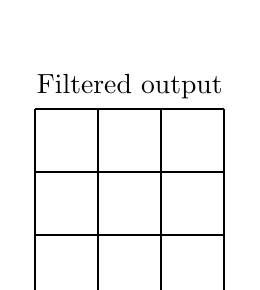
\begin{tikzpicture}[scale=.8]
\draw[step=1,thick] (0,0) grid (3,3);
\node[above] at (1.5,3){Filtered output};
\end{tikzpicture}
\end{center}
\end{studentanswer}

\end{minipage}

\item \begin{minipage}[t]{\linewidth} Describe a useful effect and a possible disadvantage of smoothing
before detecting an object. How does this fixed filter differ from filters
learned in an AlexNet-style classifier?

\begin{studentanswer}{4cm}
%%%%% SOLUTION HERE %%%%%
\end{studentanswer}

\end{minipage}

\end{enumerate}

\clearpage
\section*{Question 16: Interpreting PID and LQR responses}
The plots show illustrative position responses of the same one-axis
system to a target of 1, starting from rest at 0. The controllers use
different gains. These curves are provided for interpretation, not for
recovering numerical gains.
\begin{center}
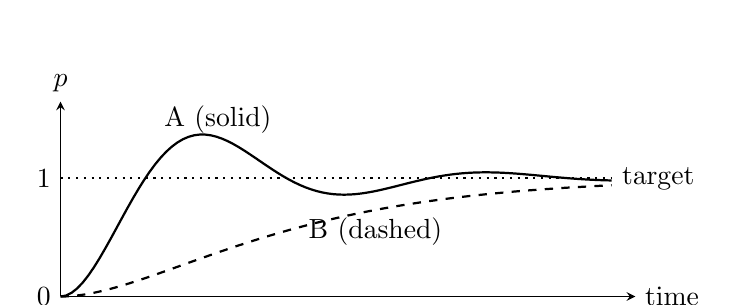
\begin{tikzpicture}[x=1cm,y=1.5cm,>=stealth]
\draw[->] (0,0)--(7.3,0) node[right]{time};
\draw[->] (0,0)--(0,1.65) node[above]{$p$};
\draw[dotted,thick] (0,1)--(7,1) node[right]{target};
\node[left] at (0,1){1}; \node[left] at (0,0){0};
\draw[thick,domain=0:7,samples=100]
 plot (\x,{1-exp(-.55*\x)*(cos(100*\x)+.315127*sin(100*\x))});
\draw[thick,dashed,domain=0:7,samples=100]
 plot (\x,{1-(1+.65*\x)*exp(-.65*\x)});
\node at (2,1.5){A (solid)};
\node at (4,.55){B (dashed)};
\end{tikzpicture}
\end{center}
\begin{enumerate}[label=(\alph*)]
\item \begin{minipage}[t]{\linewidth} Compare overshoot, oscillation, and approach to the target.
For a PID controller with zero integral gain, propose one gain change
that might reduce the oscillation in A. Explain a possible disadvantage
and why a plot alone does not identify unique gain values.

\begin{studentanswer}{4.5cm}
%%%%% SOLUTION HERE %%%%%
\end{studentanswer}

\end{minipage}
\end{enumerate}
\clearpage
\noindent\textbf{Question 16 (continued)}
\begin{enumerate}[label=(\alph*),start=2]
\item \begin{minipage}[t]{\linewidth} In a separate PID trial, a constant load opposes motion.
Integral action is disabled, and the response settles below the target.
Why can a position error remain after the motion stops? Explain what
integral action could contribute and one undesirable effect to watch for
when it is enabled. No controller equation is required.

\begin{studentanswer}{5cm}
%%%%% SOLUTION HERE %%%%%
\end{studentanswer}

\end{minipage}
\item \begin{minipage}[t]{\linewidth} A supplied LQR solver chooses gains using weights on position
error, velocity, and control effort. Compare two changes made separately
from the same initial settings: increasing the position-error weight,
and increasing the control-effort weight. Explain the intended tradeoff
in each case and propose a comparison of the resulting responses.
No objective function or gain calculation is required.

\begin{studentanswer}{5cm}
%%%%% SOLUTION HERE %%%%%
\end{studentanswer}

\end{minipage}
\end{enumerate}

\clearpage
\section*{Question 17: A reading and an occupancy prior}
A robot estimates whether one map cell is occupied. Let $O$ denote
occupied and $F$ denote free. The prior is $P(O)=0.2$, and the sensor
has $P(\texttt{hit}\mid O)=0.8$ and
$P(\texttt{hit}\mid F)=0.2$. Otherwise it reports \texttt{no hit}.
Assume that the robot's pose is known, so the observed cell is unambiguous.
\begin{enumerate}[label=(\alph*)]
\item \begin{minipage}[t]{\linewidth} The sensor reports \texttt{hit}. Use Bayes' rule to compute
$P(O\mid\texttt{hit})$. Show the prior-times-likelihood products and
their normalization. Explain why the answer is not $0.8$.

\begin{studentanswer}{4cm}
%%%%% SOLUTION HERE %%%%%
\end{studentanswer}

\end{minipage}
\item \begin{minipage}[t]{\linewidth} In a separate trial with the same original prior, the sensor
reports \texttt{no hit}. Compute the posterior occupancy probability.
State the likelihood for each hypothesis.

\begin{studentanswer}{4cm}
%%%%% SOLUTION HERE %%%%%
\end{studentanswer}

\end{minipage}
\end{enumerate}

\clearpage
\section*{Question 18: Weighting is not resampling}
Three predicted particles have prior weights $(1/2,1/4,1/4)$.
The new observation has likelihoods $(1/5,4/5,2/5)$ at their locations.
For systematic resampling, first form cumulative weights
$\mathrm{cdf}_j=\sum_{k=1}^j w_k$. Particle $j$ occupies the interval
$[\mathrm{cdf}_{j-1},\mathrm{cdf}_j)$, with $\mathrm{cdf}_0=0$.
A draw selects the particle whose interval contains it. The random offset
has already been chosen as $u_0=1/12$. Use draws $u_0$, $u_0+1/3$,
and $u_0+2/3$. This procedure copies existing particle locations.
\begin{enumerate}[label=(\alph*)]
\item \begin{minipage}[t]{\linewidth} Compute normalized posterior weights. Explain why normalizing
the likelihoods alone gives a different answer.

\begin{studentanswer}{4cm}
%%%%% SOLUTION HERE %%%%%
\end{studentanswer}

\end{minipage}

\item \begin{minipage}[t]{\linewidth} List the cumulative weights, draws, selected particles, and new
weights. Select the first cumulative weight strictly greater than each draw.
Does selecting each particle once show that the observation had no effect?

\begin{studentanswer}{4.5cm}
%%%%% SOLUTION HERE %%%%%
\end{studentanswer}

\end{minipage}

\end{enumerate}

\clearpage
\section*{Question 19: Planning with an uncertain map and pose}
A service robot has two plausible locations on opposite sides of a
wall. Its estimator reports their mean as the current position. The map
also contains a passage last observed before furniture was moved.
The robot must choose its next action.
\begin{enumerate}[label=(\alph*)]
\item \begin{minipage}[t]{\linewidth} A teammate proposes running A* from the mean and executing the
resulting path. Explain two distinct assumptions that must be checked.
Would changing A* to RRT resolve those issues by itself?

\begin{studentanswer}{4cm}
%%%%% SOLUTION HERE %%%%%
\end{studentanswer}

\end{minipage}

\item \begin{minipage}[t]{\linewidth} Propose a defensible sequence of sensing and planning decisions.
Explain where a reusable PRM or trajectory optimization might help,
and what neither supplies automatically.

\begin{studentanswer}{4.5cm}
%%%%% SOLUTION HERE %%%%%
\end{studentanswer}

\end{minipage}

\end{enumerate}

\clearpage
\section*{Question 20: Testing an imitation policy}
A policy was trained to predict an expert driver's steering command from
the car's pose. The figure shows the same policy driving from a
demonstrated starting pose (A) and a displaced starting pose (B).
After each motion, the policy receives the car's new pose and selects
the next command. Both runs use the expert's speed.

Gray curves show expert demonstrations. Dashed curves show the learned
policy, starting at the black dot. Both panels use the same scale.
\begin{center}
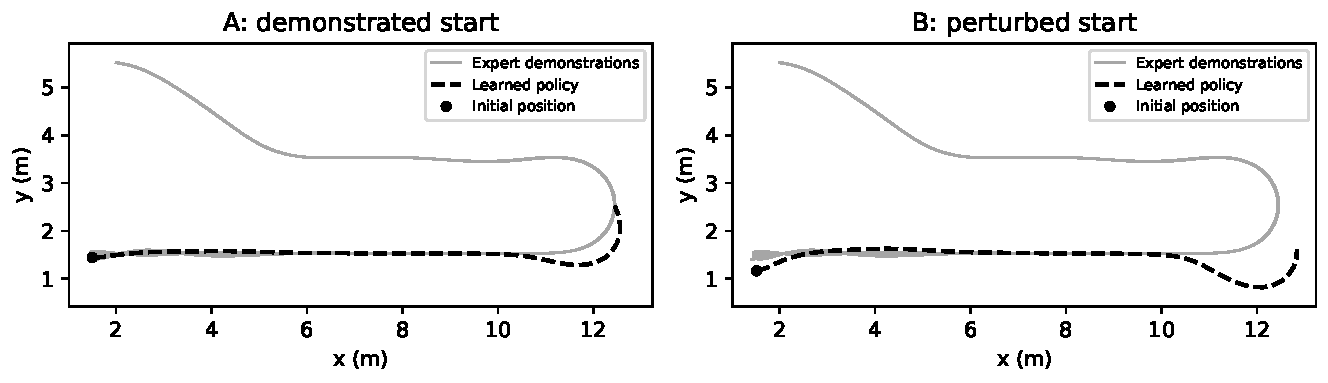
\includegraphics[width=\linewidth]{figures/imitation_walkthrough.pdf}
\end{center}
\begin{enumerate}[label=(\alph*)]
\item \begin{minipage}[t]{\linewidth} Compare the two trajectories. What does this experiment reveal
that accurate steering predictions on held-out expert poses would not?
Give one plausible explanation for the difference.

\begin{studentanswer}{4cm}
%%%%% SOLUTION HERE %%%%%
\end{studentanswer}

\end{minipage}
\item \begin{minipage}[t]{\linewidth} Would collecting more successful expert laps necessarily
address the problem? Propose one change to the training data and explain
how you would test whether it improves recovery.

\begin{studentanswer}{4cm}
%%%%% SOLUTION HERE %%%%%
\end{studentanswer}

\end{minipage}
\end{enumerate}

\clearpage
\section*{Question 21: Deployment safeguards \gradstar}
A delivery robot uses a learned policy that sometimes leaves its marked
route under unfamiliar lighting. No additional expert demonstrations can
be collected. An independent range sensor and a pose estimate are available.
A team compares three systems on the same 20 simulated routes, with the
same starting conditions and lighting changes. Each trial ends at a
collision, a completed delivery, or a fixed trial limit.

\begin{center}
\begin{tabular}{lccc}
\toprule
System & Collisions & Completed & Neither by trial limit \\
\midrule
Original policy & 8 & 12 & 0 \\
Stop on a detected deviation & 0 & 5 & 15 \\
Switch to a feedback controller & 1 & 17 & 2 \\
\bottomrule
\end{tabular}
\end{center}

\begin{enumerate}[label=(\alph*)]
\item \begin{minipage}[t]{\linewidth} Recommend one system for further testing, stating your
operating priorities. Explain what the results support and what they do
not establish. Multiple recommendations may be defensible. In particular,
does a zero in the collision column establish that the system has solved
the navigation problem?

\begin{studentanswer}{6cm}
%%%%% SOLUTION HERE %%%%%
\end{studentanswer}

\end{minipage}

\item \begin{minipage}[t]{\linewidth} Propose one modification that could improve the stopping
system's ability to finish deliveries without collecting new expert
demonstrations. State any additional information or capability it requires,
one limitation, and a test that could reveal that limitation. Do not simply
disable the stopping condition.

\begin{studentanswer}{6cm}
%%%%% SOLUTION HERE %%%%%
\end{studentanswer}

\end{minipage}
\end{enumerate}


\ifdefined\CUMULATIVEPRACTICE
\else
\end{document}
\fi
